\FloatBarrier\section{Model Predictive Control} \label{sec:mpc}

    \paragraph
    \acrfull{MPC} refers to a control system approach that determines the control action at each time-step 
    by solving an open-loop optimal control problem over a finite prediction horizon \cite{Mayne2000}.
    \gls{MPC} does not refer to a specific algorithm implementation, but rather to the general control system approach.

    \begin{figure}[ht]
        \centering
        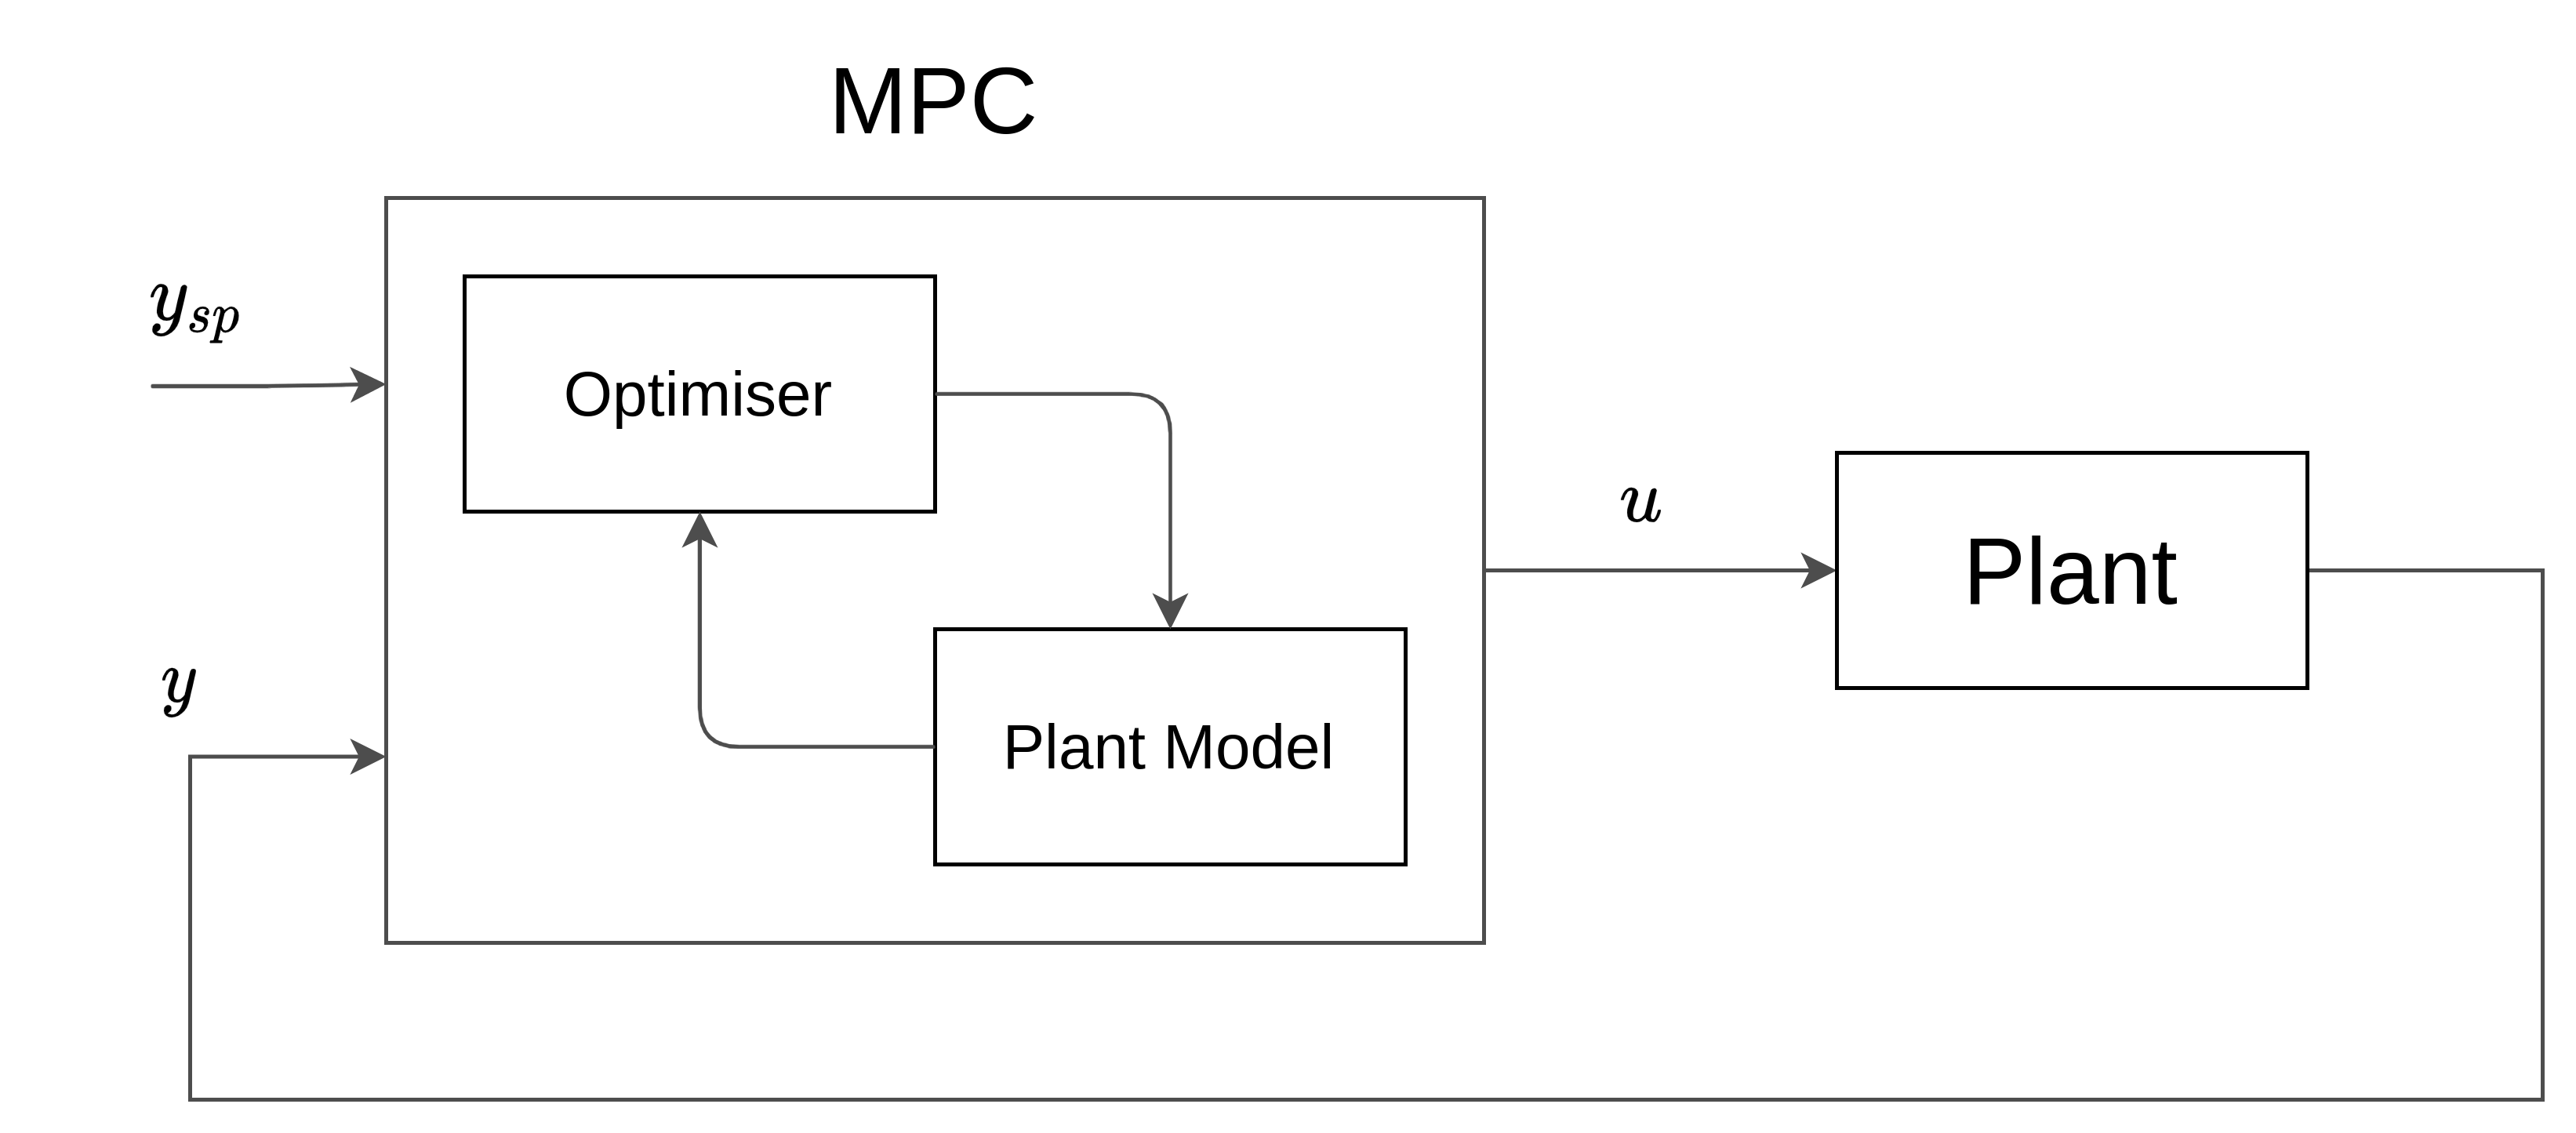
\includegraphics[width=0.818\linewidth]{control/fig/MPC_controller}
        \caption{Diagram of the structure of a typical MPC}
        \label{fig:mpc_controller}
    \end{figure}
% ?? remove all MV and MO
    \paragraph
    Figure~\ref{fig:mpc_controller} shows the structure of a typical \gls{MPC} implementation.
    As a high-level overview, the \gls{MPC} receives the measured output vector, $\bm{y}$, 
    and the output setpoint $\bm{y}_{sp}$, and determines the control action, $\bm{u}$, to drive the values in $\bm{y}$ to the values $\bm{y}_{sp}$.
    An optimiser uses an internal plant model to determine an optimal control sequence over a prediction horizon \cite{Mayne2000}.
    Therefore $\bm{y}_{sp}$ may be replaced by a target trajectory for the prediction horizon. 
    In many implementations, only the first control action of the optimal sequence is executed and the optimisation is re-calculated at every time-step.

    \paragraph
    Each specific \gls{MPC} implementation is dependant on the plant model representation \cite{Garcia1989}.
    In this section, an overview will be given of the specific \gls{MPC} implementation used in this work.
    The \gls{MPC} objective function will be explained and the design process to tune the controller will be discussed.
    It will also be discussed how integral action is achieved with the \gls{MPC}.
    Finally, the control response of the tuned \gls{MPC} will be shown and discussed for the simulated system.

    \FloatBarrier\subsection{Receding horizon}

        \paragraph
        As stated before, an \gls{MPC} considers an open-loop optimal control problem over a finite prediction horizon \cite{Mayne2000}.
        Using a plant model for predictions,
        an optimiser determines the optimal control sequence that will minimise an objective function over the prediction horizon.
        \gls{MPC} is also referred to as receding horizon control because the control sequence is determined for the next prediction horizon period at every time-step.
        
        \begin{figure}[ht]
            \centering
            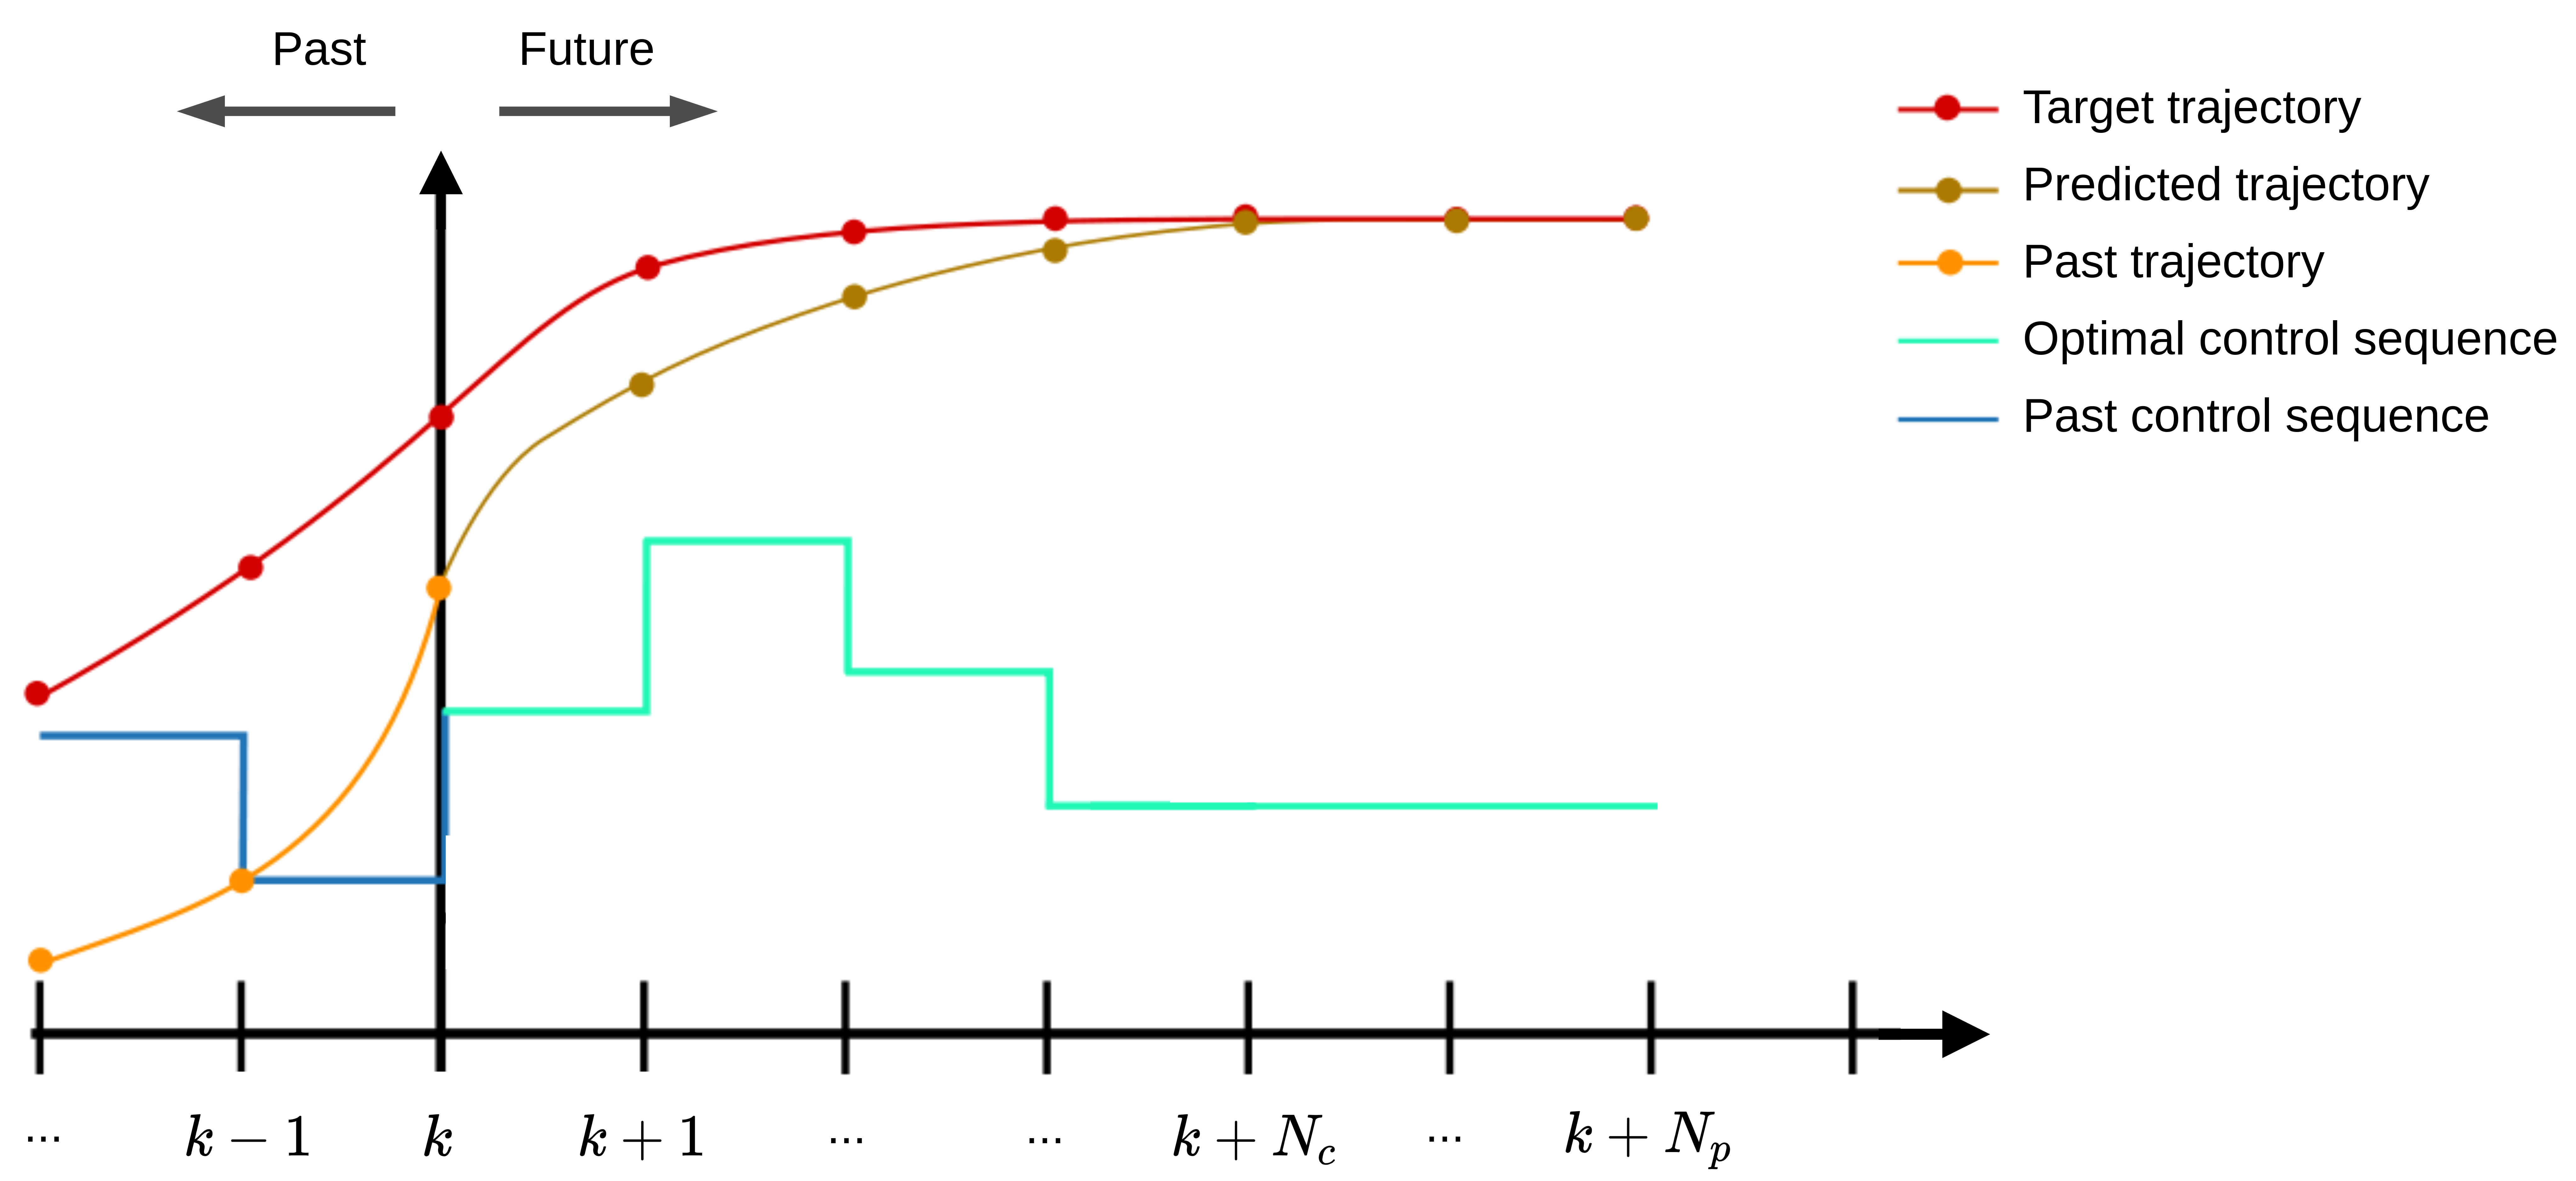
\includegraphics[width=0.818\linewidth]{control/fig/receding_horizon}
            \caption{Illustration of the receding horizon of an \gls{MPC} (adapted from \cite{horizon_diagram2021})}
            \label{fig:receding_horizon}
        \end{figure}
        
        % ?? Remove background of figure, otherwise strange outline

        \paragraph
        Figure~\ref{fig:receding_horizon} illustrates the receding horizon concept for a \gls{SISO} system.
        One of the main objectives of the optimiser is to minimise the error between the predicted trajectory and the target trajectory.
        % Therefore the \gls{MPC} determines a control sequence that would produce the optimised trajectory of the output variable.
        Starting at time-step $k$, a prediction horizon of $N_p$ time-steps is considered, and the optimiser suggests a controller decision of $N_c$ unique control values.
        $N_c$ is referred to as the control horizon and is subject to the condition, $N_c \leq N_p$.
        The control sequence, or controller decision, at time-step $k$ is denoted by,
        \begin{equation}
            {\bm{z}_k}^T = [ \bm{u}( k | k )^T ~~ \bm{u}( k+1 | k)^T ~~ ... ~~ \bm{u}( k+p-1 | k )^T ] ,
        \end{equation}
        which minimizes a specific objective function over the prediction horizon.
        The controller decision produces the predicted trajectory when applied to the plant model.
        % Note that only the first control action, $\bm{u}( k | k )$, will be executed and a new controller decision will be determined at time-step $k+1$.
        Note that if $N_c < N_p$, the remaining control actions are set to,
        \begin{equation}
            \bm{u}( i | k ) = \bm{u}( N_c | k ), ~~ i > N_c .
        \end{equation}

    \FloatBarrier\subsection{Plant model} \label{sec:mpc_model}

        \paragraph
        An important characteristic of \gls{MPC} is that it uses a separately identifiable plant model in the control optimisation process \cite{Garcia1989}.
        An estimated model from the data-driven techniques discussed in Chapter~\ref{chap:system_id} will be used as the plant model 
        for the proposed \gls{MPC} architecture.
        \gls{DMDc} produces a discrete, linear state-space model of the system dynamics.
        Hence, an \gls{MPC} implementation that corresponds to such a model will be applied.
        The following state-space model representation will be used,
        \begin{equation} \label{eq:mpc_state_space}
            \bm{x}_{mpc} (k+1) = \bm{A}_{mpc} \bm{x}_{mpc} (k) + \bm{B}_{mpc} \bm{u}_{mpc} (k) ,
        \end{equation}
        where
        $\bm{A}_{mpc}$ is the system matrix and
        $\bm{B}_{mpc}$ is the input matrix
        applied by the \gls{MPC}.
        $\bm{x}_{mpc} (k)$ is the state vector and
        $\bm{u}_{mpc} (k)$ is the input vector at time-step $k$
        for this state space model.
        It is assumed that full-state feedback is available, therefore $\bm{y}_{mpc} = \bm{x}_{mpc}$.

        \paragraph
        \gls{DMDc} applies multiple delay-coordinates to account for input delay and state delay in the system.
        In Section~\ref{sec:dmdc}, it was shown that the adapted \gls{DMDc} algorithm produces three matrices, 
        $\bm{A}_{dmd}$, 
        $\bm{A}_d$, and 
        $\bm{B}_{dmd}$.
        However, the \gls{MPC} requires a single system matrix, $\bm{A}_{mpc}$. 
        Therefore the \gls{DMDc} system is converted into:
        \begin{align}
            % 
            \begin{bmatrix}
                \bm{x}_{dmd} (k+1) \\ \bm{d} (k+1)
            \end{bmatrix}
            &=
            \begin{bmatrix}
                \bm{A}_{dmd} & \bm{0} \\
                \bm{I}_d & \bm{0}
            \end{bmatrix}
            \begin{bmatrix}
                \bm{x}_{dmd} (k) \\ \bm{d} (k)
            \end{bmatrix}
            +
            \begin{bmatrix}
                \bm{B}_{dmd} \\ \bm{0}
            \end{bmatrix}
            \bm{u}_{dmd} (k) ,
            \\ 
            \phantom{\begin{bmatrix} . \\ . \end{bmatrix}} % To get vertical spacing right
            \bm{x}_{mpc} (k+1) \hspace{7pt}
            &=
            \hspace{15pt} \bm{A}_{mpc} 
            \hspace{12pt} \cdot \hspace{5pt} \bm{x}_{mpc} (k) 
            \hspace{7pt} + 
            \hspace{7pt} \bm{B}_{mpc} 
            \hspace{1pt} \cdot \bm{u}_{mpc} (k) ,
            % 
        \end{align}
        where $\bm{I}_d$ is the identity matrix that links the corresponding entries in $[ \bm{x}_{dmd} (k) ~~ \bm{d} (k) ]^T$ to $\bm{d}(k+1)$.
        This produces large state-space matrices with many output variables (represented in $\bm{d}(k+1)$) that are necessary for state predictions but do not require setpoint tracking.
        To ignore these variables in the control optimisation, they are assigned a zero weight in the \gls{MPC} objective function.
        The objective function will be further discussed in the sections below.

        \paragraph
        Recall from Section~\ref{sec:payload_state_variable} that $\dot{\theta}$ is not used in the estimated model.
        However, as discussed in Section~\ref{sec:lqr}, it is better for a controller to minimise $\dot{\theta}$, 
        rather than $\theta$.
        This is because $\theta$ has a non-zero steady-state value during a velocity step response due to aerodynamic drag.
        The state vector is therefore augmented with the $\dot{\theta}$ variable, such that the state vector is rather defined by,
        \begin{equation}
            {\bm{x}_{mpc}}^T = 
                \begin{bmatrix}
                    V_N & \theta & \dot{\theta} & \bm{d}
                \end{bmatrix} , \phantom{~~~}
        \end{equation}
        where $\bm{d}$ is the delay state vector defined in Equation~\ref{eq:delay_vector}.
        The $\bm{A}_{mpc}$ matrix is also augmented with a Backwards Euler numerical differentiation equation, such that,
        \begin{equation}
            \dot{\theta} (k) = \frac{1}{T_s} \theta(k) - \frac{1}{T_s} \theta(k-1) 
        \end{equation}
        In this way, a weight can be applied to the $\dot{\theta}$ variable in the \gls{MPC} objective function to control this variable.
        $\bm{B}_{mpc}$ is augmented with zeros so that the state space matrix dimensions agree and so that $\bm{u}_{mpc} (k)$ does not directly influence $\dot{\theta} (k)$.

    \FloatBarrier\subsection{Algorithm implementation}

        \paragraph
        A specific algorithm needs to be selected or designed to implement \gls{MPC} in this work.
        There are numerous open-source methods available for this purpose.
        An extensive list of options is provided in the survey by \cite{Nguyen2020} and the most promising ones are summarised here.
        A custom \gls{MPC} implementation can be developed in MATLAB\textsuperscript{\textregistered} or C\texttt{++} 
        with the aid of software packages like 
        CVXGEN \cite{Mattingley2012}, 
        ACADO \cite{Houska2011},
        YALMIP \cite{Lofberg2004},
        Multi-Parametric Toolbox \cite{Herceg2013}, and
        do-mpc \cite{Lucia2017}.
        Other open-source \gls{MPC} implementations are also available as \gls{ROS} packages from work done by \cite{kamelmpc2016} or \cite{Falanga2018}.
        
        \paragraph
        The Simulink\texttrademark~implementation of an \gls{MPC} from the Model Predictive Control Toolbox\texttrademark~ \cite{MPCtoolbox2019} was selected for this work. 
        It was selected because it integrates well with our simulation environment in Simulink
        and it specifically uses a discrete state-space plant model.
        The Model Predictive Control Toolbox\texttrademark~ also supports C\texttt{++} code generation for stand-alone \gls{ROS} nodes.
        Therefore, it can integrate with the SITL implementation of PX4 and it can be run on an \gls{OBC} for practical implementations.

        % ?? Check all Simulink\texttrademark~without TM
        
        \paragraph
        The Model Predictive Control Toolbox\texttrademark ~solves the control optimisation problem as a \gls{QP} at each time interval \cite{MPCtoolbox2019}.
        To do this, it applies an active-set \gls{QP} solver using the KWIK algorithm from \cite{Schmid1994}.
        This \gls{QP} usually consists of three features, namely,
        \begin{itemize}
            \item the objective function,
            \item the constraints, and
            \item the controller decision
        \end{itemize}
        The objective function provides a scalar value that quantifies the controller performance.
        The controller decision is the set of $\bm{u}_{mpc}$ values determined by the \gls{QP} solver that minimises the objective function.
        The constraints are conditions that the controller decision should satisfy, such as bounds on $\bm{x}_{mpc}$, $\bm{u}_{mpc}$, and $\Delta\bm{u}_{mpc}$ values.

        \paragraph
        A powerful advantage of \gls{MPC} is that constraints are easily included in the optimal control implementation.
        However, constraints are not necessary for this work and will not be applied.
        This is advantageous for practical implementations because unconstrained \gls{MPC} is less computationally complex than constrained \gls{MPC}.

        \paragraph
        The objective function used by the Model Predictive Control Toolbox\texttrademark~ is documented well by the corresponding user manual \cite{MPCtoolbox2019}, and an overview of this implementation will be presented.
        The objective function consists of the sum of three terms that each quantify a specific aspect of the control performance,
        and is calculated as,
        \begin{equation} \label{eq:mpc_objective_function}
            J(\bm{z}_k) = J_y(\bm{z}_k) + J_u(\bm{z}_k) + J_{\Delta u}(\bm{z}_k),
        \end{equation}
        where $\bm{z}_k$ is the controller decision at time-step $k$.
        The three scalar performance measures are denoted as
        $J_y(\bm{z}_k)$ for output setpoint tracking,
        $J_u(\bm{z}_k)$ for \gls{MV} tracking, and
        $J_{\delta u}(\bm{z}_k)$ for \gls{MV} move suppression.
        Each performance measure includes weights that balance the competing objectives of the different terms.
        These weights need to be manually tuned for a desired controller performance.

        \paragraph
        \textbf{Output setpoint tracking}  \newline
        The performance measure of the output setpoint tracking is calculated as,
        \begin{equation}
            J_y(\bm{z}_k) = \sum_{j = 1}^{n_y} ~ \sum_{i = 1}^{N_p} 
                \left\{ 
                    {w^y}_{j} 
                        \left[ 
                            r_j( k+i | k) - y_j( k+i | k)
                        \right]
                \right\}^2 ,
        \end{equation}
        where the symbols are denoted as, \newline
        \begin{tabular}{ l l } 
            $k$             & Current control interval time-step. \\
            $n_y$           & Number of output variables. \\ 
            $N_p$           & Prediction horizon. \\ 
            $y_j( k+i | k)$ & Predicted value of $j$\textsuperscript{th} output variable at $i$\textsuperscript{th} time-step from $k$. \\
            $r_j( k+i | k)$ & Reference value of $j$\textsuperscript{th} output variable at $i$\textsuperscript{th} time-step from $k$. \\
            ${w^y}_{j}$     & Tuning weight for $j$\textsuperscript{th} output variable. \\
        \end{tabular}

        \paragraph
        The controller receives the reference values, $r_j( k+i | k)$, for the prediction horizon starting at time-step $k$.
        Using the internal plant model, the predicted output values, $y_j( k+i | k)$, is determined based on the controller decision, $\bm{z}_k$.
        The values of $N_p$ and ${w^y}_{j}$ are design choices that are constant controller specifications.
        The value of $n_y$ are also constant and are determined from the plant model.

        \paragraph
        \textbf{Manipulated variable tracking}  \newline
        In some control applications, it is desirable to keep specific \gls{MV} variables close to a target value.
        In the multirotor use case, lower \gls{MV} values are preferred because this corresponds to lower energy use.
        The \gls{MV} target values are therefore set.
        The performance measure of manipulated variable tracking is calculated as,
        \begin{equation}
            J_u(\bm{z}_k) = \sum_{j = 1}^{n_u} ~ \sum_{i = 0}^{N_p - 1} 
                \left\{ 
                    {w^u}_{j} 
                        \left[ 
                            u_j( k+i | k) - u_{j,sp}( k+i | k)
                        \right]
                \right\}^2 ,
        \end{equation}
        where the symbols are denoted as, \newline
        \begin{tabular}{ l l } 
            $n_u$           & Number of manipulated variables. \\ 
            $u_j( k+i | k)$ & Control decision of $j$\textsuperscript{th} \gls{MV} at $i$\textsuperscript{th} time-step from $k$. \\
            $u_{j,target}( k+i | k)$ & Target value of $j$\textsuperscript{th} \gls{MV} at $i$\textsuperscript{th} time-step from $k$. \\
            ${w^u}_{j}$   & Tuning weight for $j$\textsuperscript{th} \gls{MV}. \\
        \end{tabular}

        \paragraph
        The desired $u_{j,target}( k+i | k)$ values can be received for the prediction horizon starting at time-step $k$.
        However, for our use case, all $u_{j,target}( k+i | k)$ values are constant and zero.
        The value of $n_u$ is fixed by the plant model.
        The ${w^u}_{j}$ values are also constant and are determined as a design decision.
        
        \paragraph
        \textbf{Manipulated variable increment suppression}  \newline
        Large increments or moves in the \gls{MV} values are often undesirable for good control performance.
        In the multirotor use case, large increments of the acceleration \gls{MV}s result in aggressive jerks which may cause the system to go beyond the accurate domain of the linear approximation model.
        High frequency moves in the acceleration \gls{MV}s may also cause jittery flight dynamics because acceleration setpoint changes correspond to attitude changes.
        The performance measure of \gls{MV} tracking is used to penalise increments in the \gls{MV}s.
        This is calculated as,
        \begin{equation}
            J_\Delta u (\bm{z}_k) = \sum_{j = 1}^{n_u} ~ \sum_{i = 0}^{N_p - 1} 
                \left\{ 
                    {w^{\Delta u}}_{j} 
                        \left[ 
                            u_j( k+i | k) - u_j( k+i-1 | k)
                        \right]
                \right\}^2 ,
        \end{equation}
        where the symbols are denoted as, \newline
        \begin{tabular}{ l l } 
            ${w^{\delta u}}_{j}$   & Tuning weight for movement in the $j$\textsuperscript{th} \gls{MV}. \\
        \end{tabular}

        \paragraph
        The values of ${w^{\Delta u}}_{j}$ are constant and are determined as a design choice.

        \paragraph
        It is important to note the similarities and differences between the \gls{LQR} and \gls{MPC} objective functions.
        The \gls{LQR} implementation described in Section~\ref{sec:lqr}, did not included penalisation for MV increments.
        However, if $J_\Delta u (\bm{z}_k)$ is removed from Equation~\ref{eq:mpc_objective_function}, the \gls{MPC} and \gls{LQR} optimiser consider the same variables.

        \paragraph
        The \gls{LQR} optimisation corresponds to solving the unconstrained \gls{MPC} optimisation problem for $N_p = \infty$.
        However, the \gls{LQR} optimisation is run only once to determine the \gls{LQR} gain, whereas the \gls{MPC} optimisation is re-run at every time-step.
        Also note that the \gls{LQR} uses a continuous-time model, but the \gls{MPC} considered in this work uses a discrete-time model.

    \FloatBarrier\subsection{Integral action}

    % For an example of disturbance observer \gls{MPC} with multirotor: https://arxiv.org/pdf/2011.11104.pdf
        
        \paragraph
        A simple implementation of predictive control with multiple output variables does not inherently apply integral action or disturbance rejection.
        For the multirotor and suspended payload use case,
        \gls{MPC} control without integral action results in a non-zero steady-state error of the multirotor velocity, due to wind disturbance and inaccuracies in modelling the drag.
        % Due to modelling inaccuracies or disturbances, 
        % the \gls{MPC} may continually determine and execute a control action that does not drive the If the actual aerodynamics drag is more than the drag accounted for in the model.
        % In this case, zero steady-state error tracking for every output variable will not be achieved in the presence of any model inaccuracy or disturbance.
        
        % A example can be used to explain this with the multirotor system.
        % Consider the case when the multirotor is flying at steady-state velocity and the payload angle is at steady-state.
        % The \gls{MPC} controls both the multirotor velocity and the payload angle.
        % A new velocity setpoint is given that is slightly large than the current velocity.
        % The \gls{MPC} optimiser will generate a solution, $\bm{z}_k$, to accelerate slowly to the new velocity setpoint without disturbing the payload angle too much. 
        
        \paragraph
        Different methods have been proposed to apply integral action with an \gls{MPC}.
        A commonly used method involves applying an integrator to the control action determined by the \gls{MPC} \cite{Ruscio2013}.
        In this implementation, the \gls{MPC} determines the optimal control action increment, ${\Delta u_k}^*$,
        and calculates the control action, $u_k = u_{k-1} + {\Delta u_k}^*$ which is then applied.
        Hence, integral action is applied to the plant input.
        This method is also described by \cite{Mayne2000}.

        \paragraph
        Another commonly used strategy involves estimating an input disturbance that influences an output variable in the plant model \cite{Ruscio2013}.
        In this way, integral action is applied to the plant output.
        This integral action strategy will be applied in this work.
        Since integral action is required for $V_N$ in the North velocity controller,
        a disturbance model that influences $V_N$ is augmented to the input matrix.
        
        \paragraph
        The resulting state-space matrix is,
        \begin{equation} \label{eq:mpc_ud_state_space_model}
            \bm{x}_{mpc} (k+1) = 
                \bm{A}_{mpc} \bm{x}_{mpc} (k) 
                + 
                \begin{bmatrix}
                    \bm{B}_{mpc} & \bm{B_{ud}}
                \end{bmatrix}
                \begin{bmatrix}
                    \bm{u}_{mpc} (k) \\ \hat{u}_{ud}(k)
                \end{bmatrix} ,
        \end{equation}
        where
        $\bm{B_{ud}}$ is the input disturbance model and 
        $\hat{u}_{ud}$ is the estimated input disturbance value.
        The input disturbance model is designed as,
        \begin{equation}
            \bm{B_{ud}} = 
                \begin{bmatrix}
                    b_{ud} & 0 & 0 & \bm{0}
                \end{bmatrix}^T ,
        \end{equation}
        such that an input disturbance only influences $V_N$ in the state vector,
        \begin{equation}
            {\bm{x}_{mpc}}^T = 
                \begin{bmatrix}
                    V_N & \theta & \dot{\theta} & \bm{d}
                \end{bmatrix} . \phantom{~~~}
        \end{equation}
        The variable $b_{ud}$ is a tunable value that quantifies the effect of the input disturbance on $V_N$.
        This variable will be tuned in Section~\ref{sec:mpc_tuning}
        
% ?? Talk about design of value 0.1 in disturbance model

        \paragraph
        The specific value of the non-zero matrix entry in $\bm{B_{ud}}$ has only a slight effect on the control performance, hence the iterative tuning process for this value was simple.
        The value of $\hat{u}_{ud}(k)$ is estimated by the default Kalman filter estimator from the Model Predictive Control Toolbox\texttrademark. 
        This filter is based on the state-space model from Equation~\ref{eq:mpc_ud_state_space_model}.
        The value of $\hat{u}_{ud}(k)$ is then used in the \gls{QP} solver to determine the optimal control action of the \gls{MPC}.
        
        \paragraph
        It was determined from simulations with different payload parameters and disturbances that the \gls{MPC} with the default input disturbance estimator provides acceptable controller performance without additional tuning. 
        Hence, the default Kalman filter is used in the final control implementation.
        Zero steady-state error for velocity tracking was achieved for different payloads and different input disturbances, showing that integral action is achieved.
        The simulation results showing the \gls{MPC} integral action will be shown and discussed in Section~\ref{sec:control_implementation}.

        % ?? plot showing the difference between with integral action and without

    \FloatBarrier\subsection{Tuning} \label{sec:mpc_tuning}

        \paragraph
        An \gls{MPC} can easily be tuned for a range of different design requirements.
        The same general design requirements will be applied to the \gls{MPC} as to the \gls{LQR} in Section~\ref{sec:lqr}, namely,
        to produce a fast velocity response with zero steady-state error while damping the payload oscillations quickly.
        The \gls{MPC} is firstly tuned to have a similar response time to the \gls{LQR} so that the controller performances can be roughly compared.
        Thereafter, it is tuned to produce a trajectory that is as smooth as possible.

        \paragraph
        The \gls{MPC} parameters that are determined in the controller design are,
        $N_p$, 
        $N_c$, 
        $\bm{w}^y$,
        $\bm{w}^u$,
        $\bm{w}^{\Delta u}$, and
        $b_{ud}$.
        $T_s$ is fixed by the system identification phase, since the sample time of the discrete model and the controller should match.

        \paragraph
        In the controller tuning process, a large value of ${w^y}_{j}$ corresponds to aggressive control of the $j$\textsuperscript{th} output variable, 
        because the tracking error of that variable will be heavily penalised.
        In contrast, small values of ${w^u}_{j}$ or ${w^{\Delta u}}_{j}$, correspond to aggressive manoeuvres, 
        because the control values are not heavily penalised in the objective function. 

        \paragraph
        The computational complexity of the \gls{QP} problem increases significantly with larger values of $N_p$ \cite{Sawma2018}.
        % The value of $N_c$ influences the number of unique decision values in $\bm{z}_k$.
        The computational complexity also increases with larger values of $N_c$.
        Therefore the smallest values of $N_p$ and $N_c$ that still provide acceptable controller performance will be used.
        In the tuning process, the initial values were set to 
        $T_p = T_c = 2 \times t_{p}$
        where 
        $T_p = N_p \times T_s$,
        $T_c = N_c \times T_s$, and
        $t_{p}$ is the peak-time of the velocity step response with a \gls{PID} controller.
        The objective function weights were then tuned for a desired controller performance.
        
        \paragraph
        The objective function weights were iteratively tuned for the desired control performance in a similar way to the LQR.
        All the weights corresponding to the delay-coordinates are set to zero.
        Due to the non-zero steady-state value of $\theta$, the corresponding weight is also set to zero.
        Hereafter, the value of $T_p = T_c$ is incrementally decreased until a noticeable change in the controller performance.
        $T_p$ is fixed at the smallest value before this change occurs.
        $T_c$ is then further decreased until a noticeable change in performance.

        \paragraph
        The last variable to be tuned is $b_{ud}$, which influences the disturbance rejection performance of the controller.
        A large value of $b_{ud}$ results in a fast disturbance rejection performance, however, it also produces a large overshoot.
        Starting at an initial guess of $b_{ud} = 1$, the value is iteratively tuned for a consistent performance with a range of different payloads and wind disturbances.

        \paragraph
        The final designed controller configuration parameters are shown in Table~\ref{tbl:mpc_params}.
        Note that the weights in $\bm{w}^y$ correspond to the variables in, 
        $ [ V_N ~~ \theta ~~ \dot{\theta} ] $,
        the weight in $\bm{w}^u$ corresponds to the variable $A_{N_{sp}}$, and 
        the weight in $\bm{w}^{\Delta u}$ corresponds to the variable $\Delta A_{N_{sp}} (k)  =  A_{N_{sp}} (k) - A_{N_{sp}} (k-1)$.

        \begin{table}[!htbp]
            \renewcommand{\arraystretch}{1.1}
            \centering
            \caption{MPC configuration parameters.}
            \begin{tabularx}{0.3\linewidth}{@{}cc@{}}
                \toprule
                \textbf{Parameter}   & \textbf{Value} \\
                \midrule
                    $N_p$   &  166 \\
                    $N_c$   &  116 \\ 
                    $T_s$   &  \SI{0.03}{\second}\\
                    $\bm{w}^y$   &  $[ 2~~0~~10 ]$ \\
                    $\bm{w}^u$   &  $[0.1]$ \\ 
                    $\bm{w}^{\Delta u}$   & $[10]$ \\
                    $b_{ud}$ & 0.1 \\
                \bottomrule
            \end{tabularx}
            \label{tbl:mpc_params}
        \end{table}

        \begin{figure}[htb]
    \centering
    \begin{tikzpicture}
        \begin{axis}[            
            xlabel = Time,
            ylabel = North velocity,
            x unit = \si{\second},
            y unit = \si{\metre/\second},
            xmin = 0,   xmax = 16,
            ymin = -0.1,  ymax = 2.4,
            grid = major,
            legend cell align = left,
            legend pos = south east,
            grid style = dashed,
            legend style = {font = \scriptsize},
            label style = {font = \scriptsize},
            tick label style = {font = \scriptsize},
            width = 0.95\columnwidth,
            height = 0.5\columnwidth,
            % initialize Dark2
            cycle list/Dark2,
            % combine it with 'mark list*':
            cycle multiindex* list = {
                Dark2\nextlist
            }
        ]
        
        \addplot+[mark = none, style = solid, ultra thick] 
        table[x = time, y = vel_sp, col sep = comma] 
        {control/csv/compare_control_mpc_Simulink_single_pend_mp0.3_l2.25_MPC_vel_steps_tune_scale_0.7.csv};
        \addlegendentry{Setpoint}

        \addplot+[mark = none, style = solid, ultra thick] 
        table[x = time, y = vel, col sep = comma] 
        {control/csv/compare_control_mpc_Simulink_single_pend_mp0.1_l0.5_MPC_vel_steps_tune_scale_0.7.csv};
        \addlegendentry{($l =$~\SI{0.5}{\meter}, $m_p =$~\SI{0.1}{\kilo\gram})}

        \addplot+[mark = none, style = solid, ultra thick] 
        table[x = time, y = vel, col sep = comma] 
        {control/csv/compare_control_mpc_Simulink_single_pend_mp0.2_l1_MPC_vel_steps_tune_scale_0.7.csv};
        \addlegendentry{($l =$~\SI{1}{\meter}, $m_p =$~\SI{0.2}{\kilo\gram})}

        \addplot+[mark = none, style = solid, ultra thick] 
        table[x = time, y = vel, col sep = comma] 
        {control/csv/compare_control_mpc_Simulink_single_pend_mp0.3_l2.25_MPC_vel_steps_tune_scale_0.7.csv};
        \addlegendentry{($l =$~\SI{2}{\meter}, $m_p =$~\SI{0.3}{\kilo\gram})}

        \end{axis}
    \end{tikzpicture} 
    \caption{\gls{MPC} velocity step responses with different payloads}
    \label{fig:mpc_tuning_plot}
\end{figure}


        \paragraph
        Figure~\ref{fig:mpc_tuning_plot} shows a plot of the simulated \gls{MPC} velocity response with different payload parameters.
        It is clear that the controller damps the payload angles well and produces a smooth trajectory with different payloads.
        For each different payload, a \gls{DMDc} model is first estimated.
        Thereafter the \gls{MPC} is simulated with the same controller configuration defined in Table~\ref{tbl:mpc_params}.
    
